\section{McG Experiment Result} 
In this section, we will discuss the results from running the market in full McG action-step system with all the agents. Similar to Oesch, McG does not fully state the ratio of the agents nor the number in each run. McG only reported their results as return statistics and price spikes data. In addition, because of hardware limitation and time-constraint, we will only be testing the McG experiment with 100,000 maximum time-step since running 300,000 takes at least 7 hours on our personal computer and the increase in time-period does not change the market dynamics. 

\subsection{Changes to Mean reversion and Momentum traders}
Upon investigation, the Mean reversion and Momentum trader seems to be submitting less than ideal orders and quantity of the orders compared to the other agents. In a 30,000 action-step in testing, the agents occasionally submit lower than 10,000 quantity or does not submit any orders at all. This means that some changes needed to be made to the agents in order to adapt them to the market. 

\begin{table}[h]
\centering
\begin{tabular}{ |m||p{4cm}|p{4cm}|} 
\hline
\textbf{Agent Parameter}& \textbf{ Original Value } & \textbf{New Value} \\
\hline
\hline
Momentum Trader's Wealth $W_{a,t}$ & 500,000 & 1,000,000  \\ 
\hline
Mean Reversion quantity per order $V_{mr}$ & 1 & $U(1, 5000)$ \\ 
\hline
\end{tabular}
\label{Tab:C5_parameters}
\caption{Changes in parameters of Mean Reversion trader and Momentum trader}  
\end{table}
\FloatBarrier

Because McG does not specify how to calculate the wealth of the Momentum trader, a choice has to be made regarding its initial wealth. In a 10,000 action-step, 500,000 worked well with the initial test since the total time period is smaller. However, since the current time period is higher, the wealth has to be increase in order to make the agent participate for the whole period without losing much of its wealth as well as submitting an increasing quantity of orders. 

For the Mean reversion trader, the quantity described by McG does not make sense since other agents are submitting more than 1 orders in most cases. The new change specifies that the Mean reversion trader will submit an order quantity uniformly distributed from 1 to 5,000. This number is taken from the average quantity that change make a shift of 0.05\% of mid price. A small experiment is conducted where a market of all five agents ran and recorded a shift in price when an order is submitted of more than 0.05\% from the initial price. The average of quantity of said order is 5,000. 

This change is crucial because in the next section where \textbf{Price Spike} is explained, the two agents, Mean reversion and Momentum trader will have an opposite behaviour in terms of types of orders submitted compared to one another. Hence, it does not make sense in this case where one will submit large quantities in an order while the other only submits orders of one quantity. 

In addition, McG specifies that Mean reversion agent has an effect on the mid-price and quantity of one is far too small to have an effect. Another possible change is to increase the number of Mean reversion agents in order to make the their orders have a larger effect on the market. 

The reason why these agents need to have a larger effect on the market is because McG market has a special property that mimics the real market dynamic called \textbf{Price Spikes}.

\subsection{Price Spike}

Taken from Johnson et al., McG describes a price spike as ``an occurrence of a stock price ticking down [up] at least ten times before ticking up [down] and with a price change exceeding 0.8\% of the initial price" \cite{McGroarty} McG claims that a Price Spike can occur when an agent ``eats through" the best price of one side of a book, causing a change in the mid-price of the market. This creates an upward or downward curve. Because there is a change in the mid-price, Momentum traders will now submit on the same side of the book, which pushes the price down the same direction. Mean Reversion trader, on the other hand, will detect a change in the mid-price and expects the price to shift back to its original moving average, hence will submit on the opposite side of the book. This means that there will be now roughly equal number of bids and sells which will stabilizes the mid price up to a certain point and stop the price from moving in the original direction. At this point, the Momentum trader may run no longer detect a large ROC and stop submitting. In addition, there will be another trader which will eat through the new higher or lower best price, causing a shift in the opposite direction of the original shift in price. 

\begin{figure}[h]
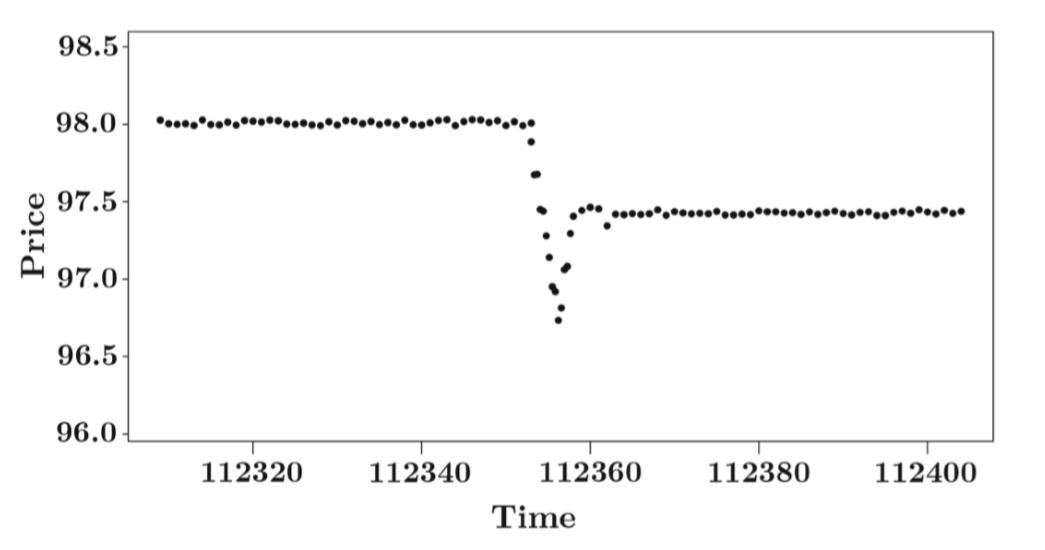
\includegraphics[ height=8cm]{Dissertation/images/Mcg_final/price_spike.PNG}
\caption{Price Spike example from \cite{McGroarty}}  
\end{figure} 
\FloatBarrier

In the current configuration, we were not able to detect a price-spike but there are other minor events which will be called \textbf{Minor Price Spikes} that exhibits the behaviour and relationship between Mean Reverison trader and Momentum trader. 

\subsection{Minor Price Spike}

A minor price spike can be defined as follow : An occurrence of price ticking up or down at least 5 times  with the maximum price of the ticks exceeding 0.6\% of the initial price. The event must happen in more than 5 action-steps. 

An example is given below: 
\begin{figure}[h]
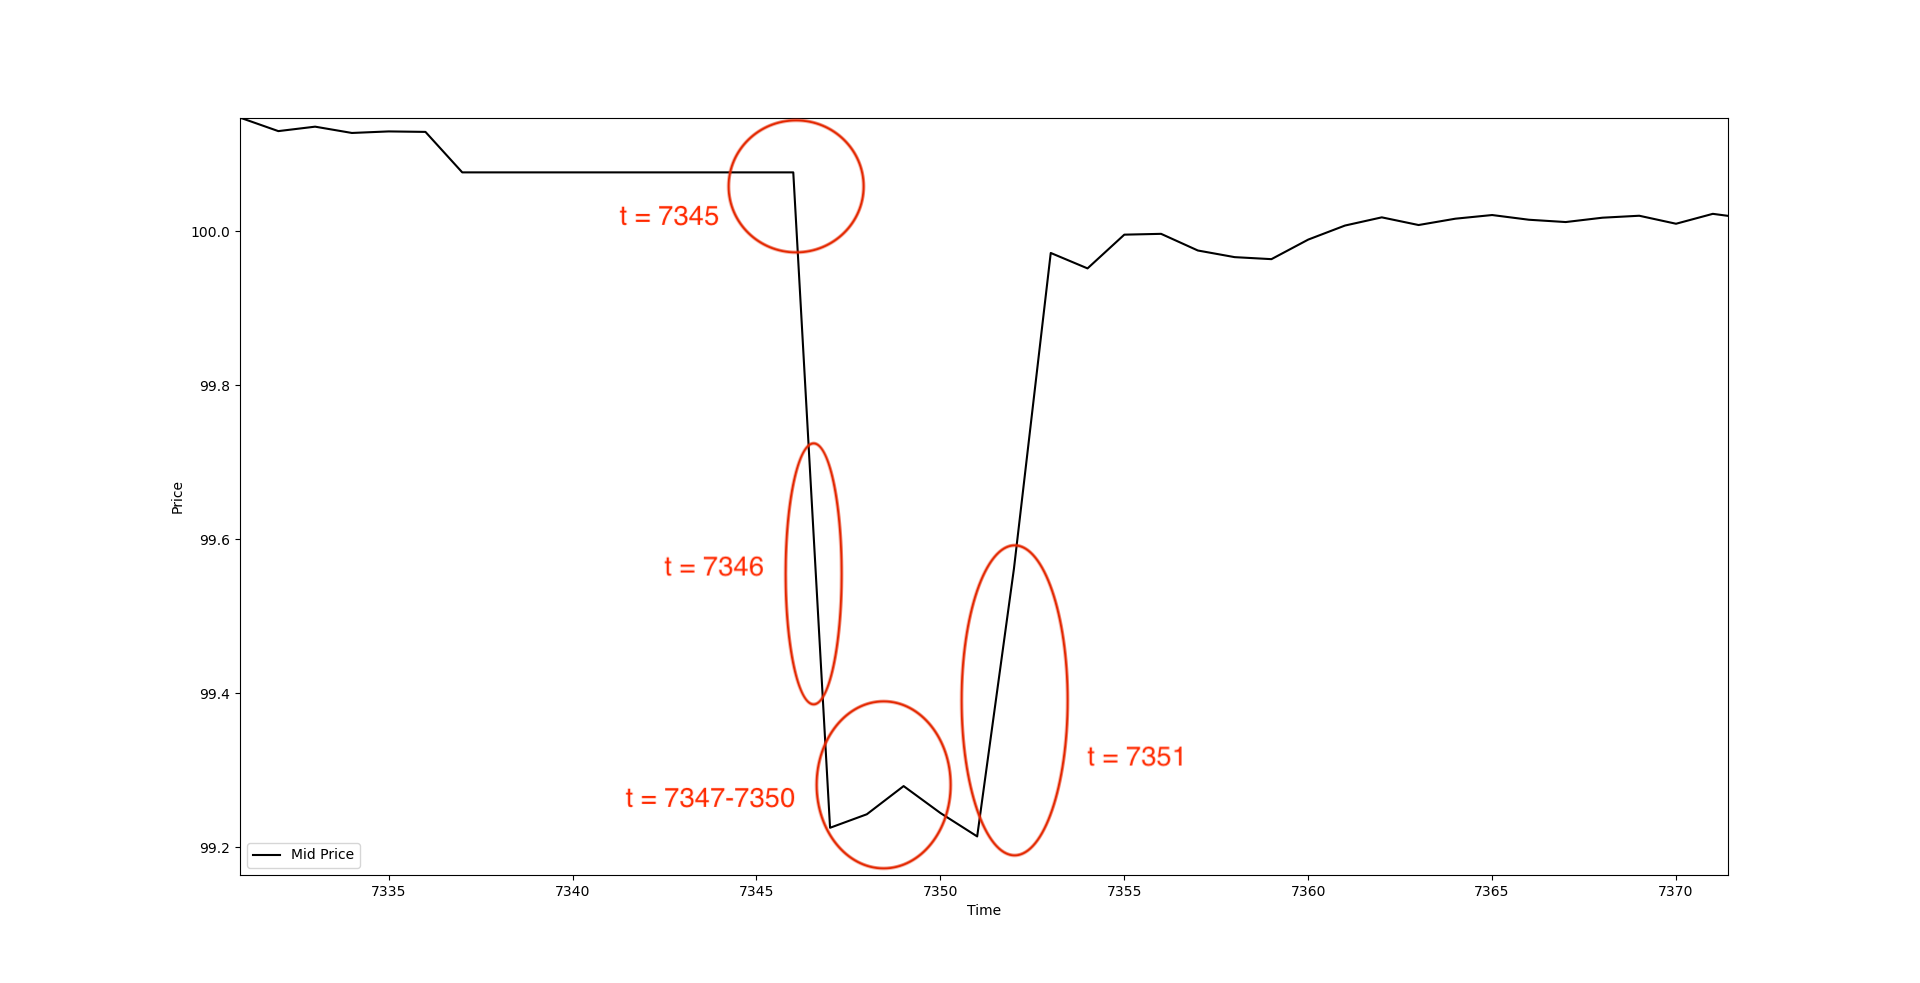
\includegraphics[ height=8cm]{Dissertation/images/Mcg_final/minor_spike_example.png}
\caption{Price spike example from the experiments}  
\end{figure} 
\FloatBarrier

A detailed explanation of the example spike: 
\begin{itemize}
  \item $ t = 7345$ A Market maker eats through the best price, causing the shift in the mid price of the market. 
  \item $ t = 7346 $ Mean reversion agents submits Bid orders while other agents, including Momentum trader, submit Ask orders causing the price to shift even downwards. Since there are more Ask order submitted, the price shifts downwards to 99.2. 
  \item $ t = 7347-7350 $ Mean reversion now submits an Ask order since the $ema_t$ value sees a small shift upward in price and because the McG value of 0.94 accounts to the change in the last 2 action-step price. However, the quantity is small since only a small portion of the agents are submitting. On the other hand, because there is still momentum from the last 5 action steps of a downward shift in price, the Momentum trader still submits Ask orders, but with less quantity, causing a smaller downward slope in the mid-price. 
  \item $ t = 7351 $ An agent again ``eats through" the best price, causing the mid price to shift upwards to 99.9. This causes the Momentum trader to submit bid orders while Mean reversion agent submits Ask orders. 
\end{itemize}

\section{Parameters and Minor Price Spike}
Now that there we have established the relationship between the Mean reversion and Momentum trader, the changes in parameter can also affect the number of minor spikes seen in the market. In this section, we will explore how the parameters of each trading agent, more specifically parameters that relate to their reaction to the market in terms of time-period and how these parameters effect the number of Minor Price Spikes found in each experiment. In addition, McG states in their paper that as the number of frequency trader increases, more price spikes can be seen \cite{McGroarty}. This can be shown with the number of Minor Price Spikes in our experiments, which will be illustrated in Table 6.4 below. 

\subsection{Threshold of Momentum trader and Number of Minor Price Spike recorded}

\begin{algorithm}[H]
\DontPrintSemicolon 
\If{$random() < \delta_{mt}$} {
    \If{$roc_t \ge \kappa$} {
    Submit market buy order with volume $v_t = \abs{roc_t} * W_{a,t}$\;
    }
    \uElseIf{$roc_t \leq -\kappa$}{
    Submit market sell order with volume $v_t = \abs{roc_t} * W_{a,t}$;\
    }
    \EndIf
  }
\EndIf
Update ROC $roc_t = \frac{p_t - p_{t-n_r}}{p_{t-n_r}}$\;  
\caption{{\sc Momentum trader reproduced from McG (4.3) \cite{McGroarty} } }
\label{algo:max}
\end{algorithm}

By decreasing the threshold of the Momentum trader threshold $\kappa $ in Algorithm 6.1 above from 0.001 to 0.0001, this means that the trader will react to smaller changes in the mid-price hence will submit more orders. Because there are more orders from the trader, it is obvious that there will be more Minor Price Spikes throughout the experiments as shown in Table 6.2 where the average of Minor Price Spikes seen increase from 0.57 to 0.75. 

\begin{table}[h]
\centering  
\begin{tabular}{ |m||p{2cm}|p{2cm}|p{2cm}|} 
\hline
\textbf{Market Configuration}& \textbf{ Min } & \textbf{ Mean } & \textbf{ Max}\\
\hline
\hline
Original parameter & 0 & 0.57 & 2 \\ 
\hline
Decreasing Momentum trader threshold 0.0001 & 0 & 0.75 & 2 \\ 
\hline 
\hline
\end{tabular}
\label{Tab:6.2}
\caption{Minor Price Spikes statistics with change in Momentum trader threshold $\kappa$}  
\end{table}
\FloatBarrier

\subsection{Threshold of Mean Reversion trader and Number of Minor Price Spike recorded}

\begin{algorithm}[H]
\DontPrintSemicolon 
\If{$random() < \delta_{mr}$} {
    \If{$p_t - ema_t \ge k\sigma_t$} {
    Submit sell just inside best ask with $v_t = v_{mr}$\;
    }
    \uElseIf{$ema_t - p_t \ge k\sigma_t$}{
    Submit buy just inside best ask with $v_t = v_{mr}$\;
    }
    \EndIf
  }
\EndIf
Update $ema_t$ = $ema_{(t-1)} - \alpha(p_t - ema_{(t-1)}$
\caption{{\sc Mean reversion trader reproduced from McG (4.4) \cite{McGroarty}} }
\label{algo:max}
\end{algorithm}

Previous results suggest that these Minor Price Spikes often occur in around 5 action-steps, which is why we experimented with changing the Mean Reversion trader's equation and parameter $\alpha$ from 0.94 to 0.33 which accounts to the last $n = 5$ action-step changes in price instead of $n = 1.1$ as previously calculated in Chapter 4.4.

\begin{equation}
ema_t = (p_{t} - ema_{t-1}) * (2 / n + 1) + ema_{t-1} 
\end{equation}
where n = period.

In addition, this is also switching from the McG equation to the equation 6.1. Statistics in Table 6.3 illustrates that by making Mean Reversion trader's period much smaller, it is more likely to submit more orders when there are recently large increase or decrease in price hence increases the average of Minor Price Spike seen in one experiment increases from 0.57 to 2.  

\begin{table}[h]
\centering  
\begin{tabular}{ |m||p{2cm}|p{2cm}|p{2cm}|} 
\hline
\textbf{Market Configuration}& \textbf{ Min } & \textbf{ Mean } & \textbf{ Max}\\
\hline
\hline
Original parameter & 0 & 0.57 & 2 \\ 
\hline
Change in Mean Reversion parameter & 0 & 2 & 3 \\ 
\hline 
\hline
\end{tabular}
\caption{Minor Price Spikes statistics with change in Mean Reversion trader threshold equation and period}  
\end{table}
\FloatBarrier

\subsection{Ratio of frequency traders and Number of Minor Price Spike recorded}
McG explained in their findings that ``increasing the total number of high frequency participants ... do lead to an increase in price spike events" \cite{McGroarty}. Hence, we also experimented with the ratio of the two high frequency trader (Momentum trader and Mean Reversion trader) compared to other types of agents. Table 6.4 illustrates the Minor Price Spikes event statistics in our experiments where we find a similar pattern to McG. By increasing the frequency traders to twice and three times that of other agents, there is a clear increase in the number of Minor Price Spike detected where a including two times more frequency than other agents lead to an increase from 0.57 to 0.9 on average per experiment and 0.57 to 2.7 in the case where there are three times more frequency traders. 

\begin{table}[h]
\centering  
\begin{tabular}{ |m||p{2cm}|p{2cm}|p{2cm}|} 
\hline
\textbf{Market Configuration}& \textbf{ Min } & \textbf{ Mean } & \textbf{ Max}\\
\hline
\hline
Original parameter & 0 & 0.57 & 2 \\ 
\hline
2:1 ratio of high frequency trader and other traders & 0 & 0.9 & 3 \\ 
\hline 
3:1 ratio of high frequency trader and other traders & 0 & 2.7 & 5 \\ 
\hline 
\hline
\end{tabular}
\caption{Minor Price Spikes statistics with different ratio of high frequency traders}  
\end{table}
\FloatBarrier

\newpage
\section{McG full market experiment results}
\subsection{Number of agents in the market and mid-price pattern}
In this experiment, we set all the number of each type of agents to the same amount so that it will illustrate the market dynamics. 

\begin{figure}[hbt!]
  \begin{subfigure}[b]{0.5\textwidth}
    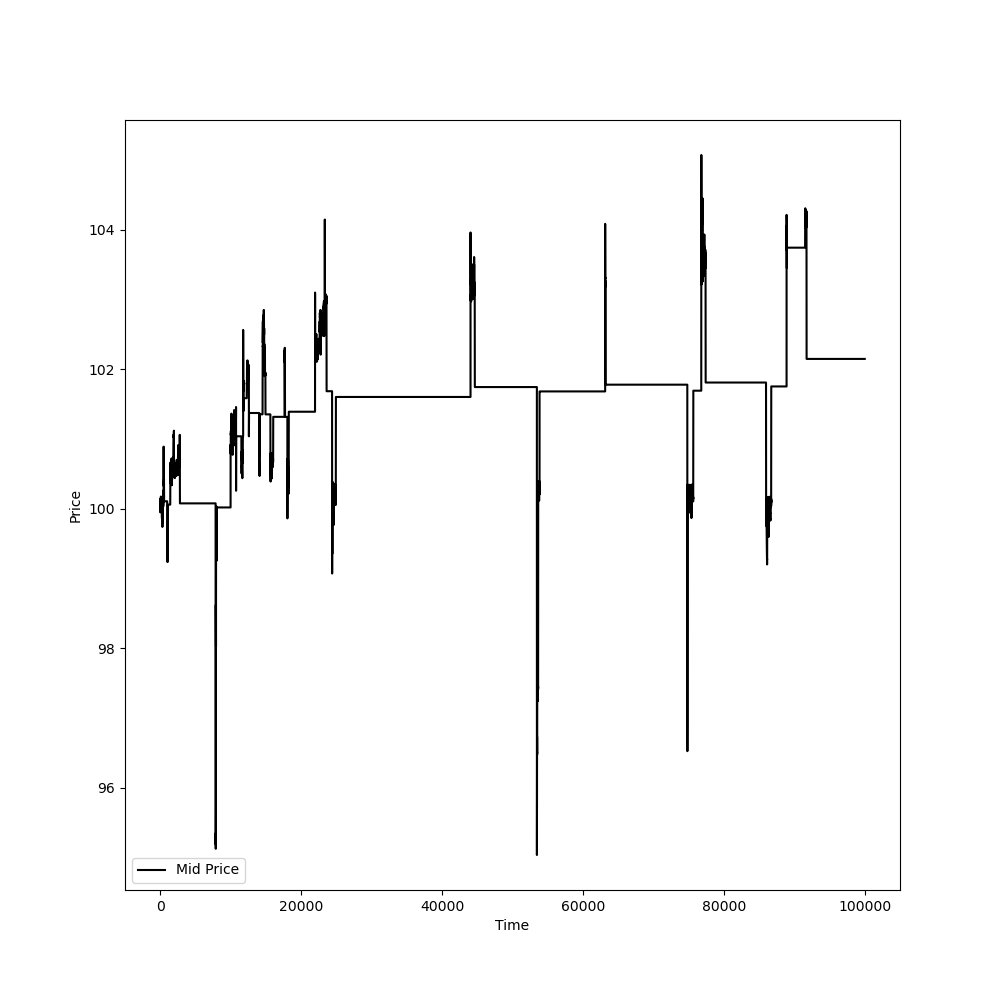
\includegraphics[width=7cm, height=7cm]{Dissertation/images/Mcg_final/full/mcg_10.png}
    \caption{20 of each agent}
    \label{fig:mcg_all_20}
  \end{subfigure}
  %
  \begin{subfigure}[b]{0.5\textwidth}
    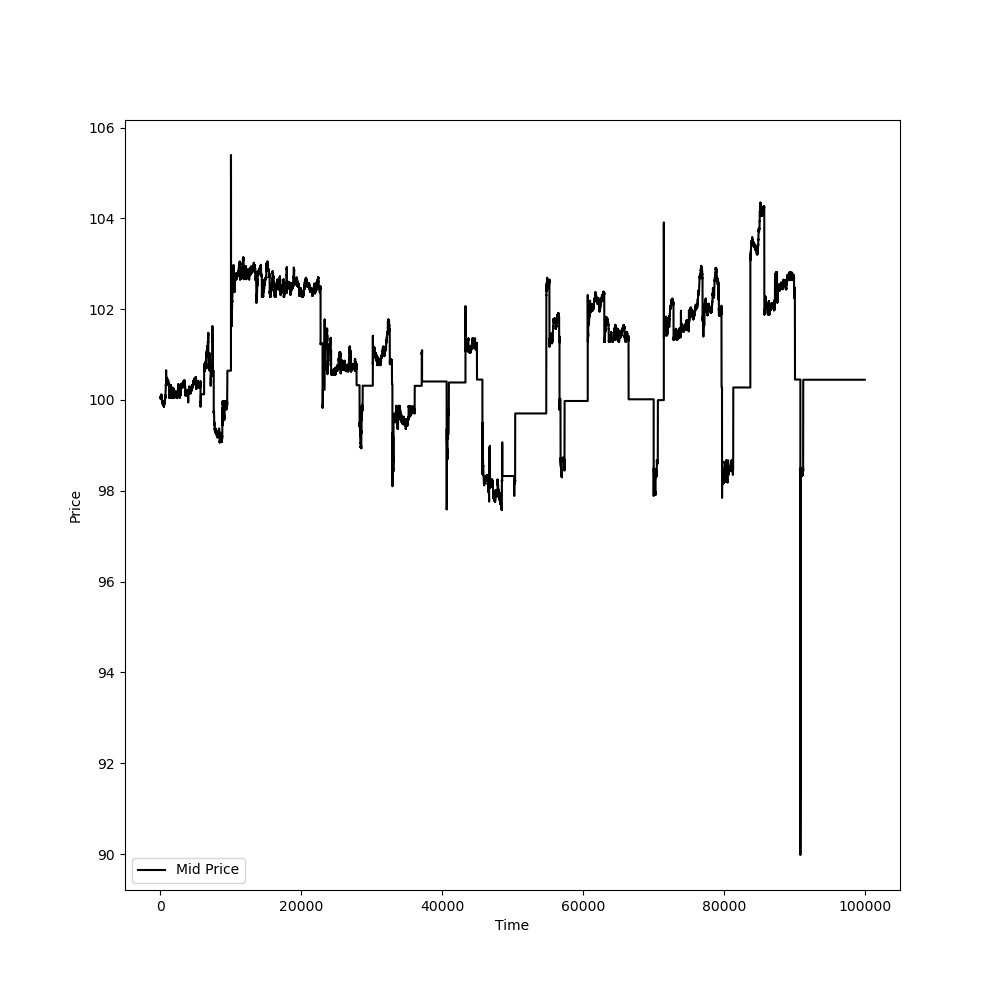
\includegraphics[width= 7cm, height= 7cm]{Dissertation/images/Mcg_final/full/mcg-20.png}
    \caption{40 of each agent}
    \label{fig:mcg_all_40}
  \end{subfigure}

  \begin{subfigure}[b]{0.5\textwidth}
    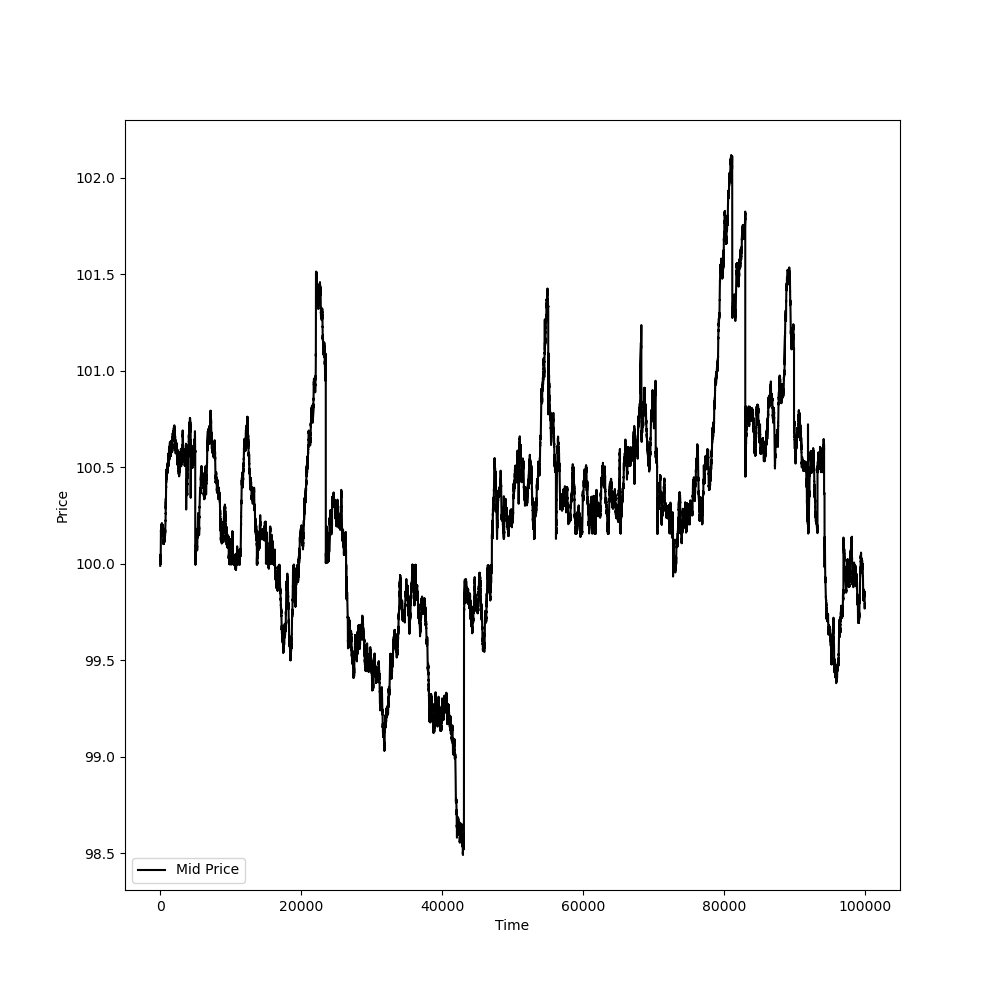
\includegraphics[width=7cm, height=7cm]{Dissertation/images/Mcg_final/full/mcg-30.png}   
    \caption{60 of each agent}
    \label{fig:mcg_all_60}
  \end{subfigure}
  %
  \begin{subfigure}[b]{0.5\textwidth}
    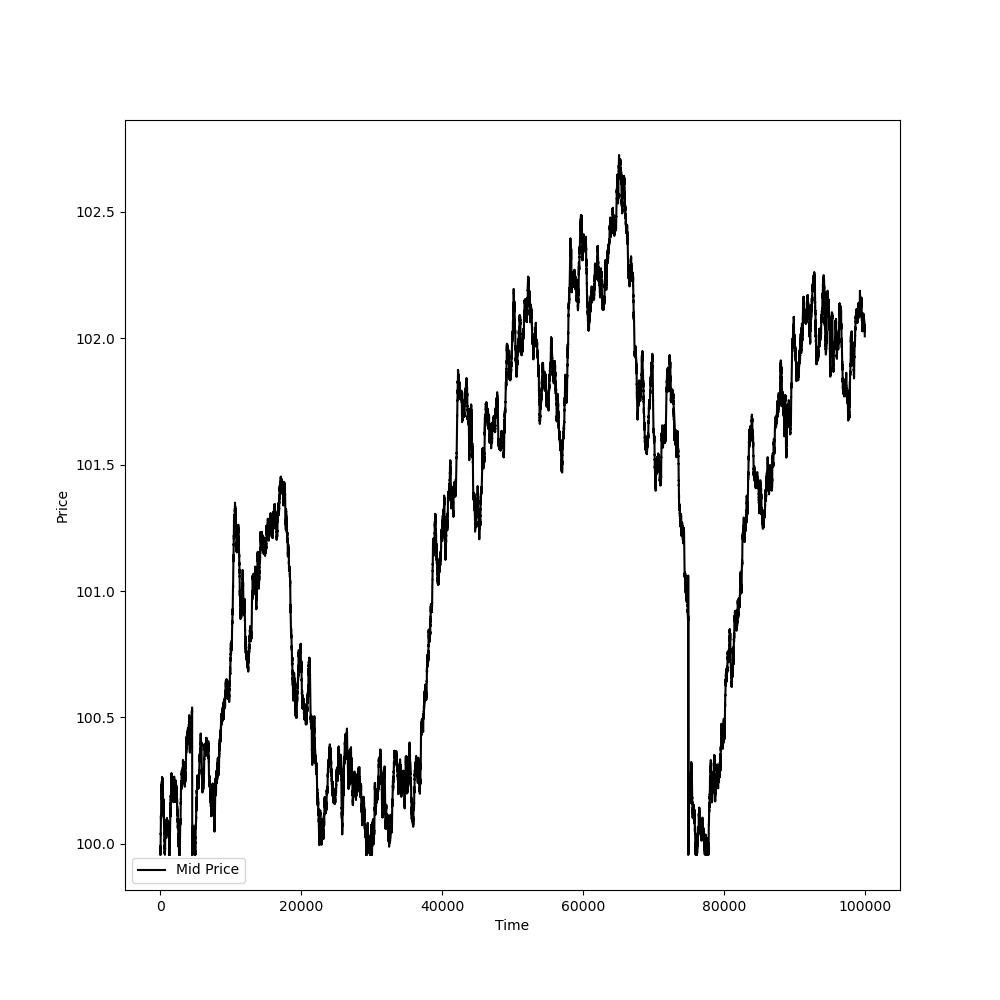
\includegraphics[width= 7cm, height= 7cm]{Dissertation/images/Mcg_final/full/mcg-40.png}
    \caption{80 of each agent}
    \label{fig:mcg_all_80}
  \end{subfigure}
\caption{Mid price Series of different number of agents in the market ran with 100,000 McG action-step} 
\end{figure}
\FloatBarrier

Similar to what we found with Oesch's market, In Figure \ref{fig:mcg_all_20} and Figure \ref{fig:mcg_all_40} when there are small number of agents in the market, we experience a market where there are unrealistic price patterns caused by the lack of Noise agents and unrealistic price spikes caused by Market maker and Liquidity consumer submitting large orders. On the other hand in Figure \ref{fig:mcg_all_80}, when there are a lot of agents in the market, the price will not cross the initial mid price and moves toward one direction over the whole experiment period with agents submitting at the best price moving it to one direction. 

\subsection{Noise agent and its crucial role in the simulated market}

Another interesting but not obvious result is that if there are no Noise agents in the market, the behaviour will not be as expected. Without the Noise agent, the mid-price of the whole market will be a flat line, regardless of the time-period of the experiment. This comes from a number of reasons: 

\begin{itemize}
  \item Mean Reversion trader will not submit an orders because there is no change in the value of the price, hence the standard deviation will be 0. This means that the price will already be at the moving average and will not trigger any conditions that the Mean reversion trader will submit an order.
  \item Momentum trader will also submit no orders because there is no change in price, hence no change in the momentum of the price. 
  \item This leads to the fact that only Liquidity consumer and Market maker that will submit orders. Liquidity consumer only submit market orders, hence no change in price will accord from its orders. Market maker only submits at best price, and since there are no other agents that will contribute to the change in price, there will be no deviation from the initial best price of the market. 
\end{itemize}

\section{Evaluation of Results}

\subsection{Oesch's configuration experiments}
In Chapter 5 we have successfully simulate a market in which the price pattern is in range of the original literature as well as a close mid-price return pattern. By doing this, we achieved part of our original goal which is implement the 3 out of 5 trading agents that Oesch's original paper claims to produce real market dynamics. In section 5.1.2 and 5.1.3, we also explored how the number of agents in the market and the price patterns in each market configuration. This gave us a better insight on the behaviour of Market makers and Liquidity consumer and how they react in different market conditions. In addition, in section 5.1.4 we also explored how the ratio of Noise agent in the market affects the price pattern and how it can create an unrealistic price pattern if there are less of them in the market. 

Overall, Chapter 5 provides us with a better insight on the three agents : Noise trader, Market maker and Liquidity consumer. However, there are areas that we would like to explore in the future. In Oesch's original conference paper, the literature took a deeper look into price impact on the market. This can be described as ``Market or price impact is the effect a trade has on the market price of a financial asset. An executed sell (buy) trade is usually associated with a fall (rise) in the market price." \cite{Oesch}. Oesch took a deeper look into how the ratio of these traders as well as how parameters of each agent affect the price impact function. Although this is a very interesting topic that we would like to explore, on top of return statistics analysis such as Kurtosis and volatility clustering which can be described as ``large changes in price tend to follow other large price changes" \cite{McGroarty}, it is beyond scope of this project due to time constraint. 

\subsection{McG configuration experiments}
In Chapter 6, we explored more deeply into the two frequency traders since we have established that the behaviour of the three traders can produce a similar price pattern compared with Oesch's original paper. In section 6.1.1, we explore how parameters should be adapt in order to properly implement the two frequency traders. In section 6.1.2, we explored the concept of price spikes from Johnson et al. \cite{Johnson} and McG\cite{McGroarty} where unfortunately, we were not able to mimic a price spike that is seen in the real market but did manage to reproduced the same behaviour between Mean Reversion trader and Momentum trader that causes the price spikes described in McG. 

In short, Chapter 6 provides us with a chance to explore the parameters and one of the unique feature of McG market that makes up a realistic market dynamics. In our perspective, we reached our goal for the project by implementing and adapt the McG agents so that they work with the BSE and was able to produce results that suggest the agents have similar behaviour to what is described in previous literature. This is consistent with our results in Chapter 3 and Chapter 4 where we tested the BSE integrity by comparing ZI-P, ZI-C and Sniper's behaviour with previous literature and Base Line results as well as the behaviour of individual agents to what is described in McG and Oesch. 

There are certainly interesting areas that could be improved and explored in detail in this project. The first is how close the final configuration is to McG. Because some parameters of McG were not given such as ratio of the agent and wealth calculation of the Momentum agent, it is possible that our implementation and McG's is different which outputs different values in the experiments. With more exploration, these parameters could certainly be improved with more experiments and exploration on the parameters effect on the market. In addition, although we were not able to mimic a full price-spike, the behaviour of Mean Reversion trader and Momentum trader is similar to what is described  in McG. With a deeper exploration into the parameters of the agent, a price spike can certainly be achieved. These are all areas that are beyond the scope due to the current time limit but are very interesting extensions for the current project. 